%%%%%%%%%%  End-term report, PYD411, 2026--27 Semester I  %%%%%%%%%%%%%%%%%%%%
% Compile from this directory with: pdflatex SPCP_2023PH10741_2601PYD411_ER.tex
% The PDF must be submitted as SPCP_2023PH10741_2601PYD411_ER.pdf
\documentclass[11pt]{article}
\voffset=-2.8cm
\hoffset=-1.6cm
\textwidth=14.5cm
\textheight=24.5cm
\usepackage{amsmath}
\usepackage{amsfonts}
\usepackage{amssymb}
%\usepackage{subfig}
\usepackage{epsfig}
\usepackage{hyperref}
%\usepackage[utf8]{inputenc}
%\usepackage{mathtools}
\usepackage[caption=false]{subfig}
\usepackage{soul,xcolor}


%\vspace*{-2cm}
%%%%%%%%%%%%%%%%%%%%%%%%%%%%%%%%%%%%%%%%%%%%%%%%%%%%%%%%%%%%%%%%%%%
\begin{document}
%%%%%%%%%%%%%%%%%%%%%%%%%%%%%%%%%%%%%%%%%%%%%%%%%%%%%%%%%%%%%%%%%%%
\thispagestyle{empty}
\begin{center}
 
\includegraphics[height=2.8cm,angle=0]{Logo-IITD.jpg}\\
\textbf{Dept of Physics, IIT Delhi}
\end{center}

\vspace*{0.25cm}
\begin{center}
\textbf{Course Code : PYD411}\\
\textbf{Academic Year : 2026 - 2027,\, Semester - I}\\
\end{center}

\vspace*{0.3cm}
\begin{center}
\textbf{\Huge{Phase-Field Modelling of Crawling Cells}}\\[0.2cm]
\textbf{\Large{From a Single Cell to a Two-Cell Collision}}
\end{center}

\vspace*{0.3cm}
\begin{center}
\textbf{\Large{Siddharth Kumar (2023PH10741)}}\\
\textbf{\Large{Soumik Roy (2023PH10756)}}\\
\end{center}

\vspace*{0.25cm}
\begin{center}
\textbf{\Large{Adviser: Prof. Sujin B. Babu}}\\
\end{center}

\vspace*{0.3cm}
\noindent
\textbf{Abstract}: We implement a continuum phase-field model of a crawling cell, following Tjhung et al.\ and the effective-friction picture of substrate adhesion, and then extend it to two cells that can meet. The model is built in four single-cell stages so that each ingredient can be isolated. Without flow a cell translates but loses 4.5\% of its area. Confining treadmilling to a layer at a wall produces a leading protrusion. The full planar model, with Stokes flow, active stress and anchoring, recovers the non-motile aster and the lamellipodial fan; in this geometry the shape is set by anchoring, and the flow adds about 2\%. Replacing the Stokes solve by its friction-dominated limit gives a cell that crawls steadily, at speed 0.801, and is local enough to be repeated. For two cells each cell keeps its own phase field and polarization, and the two forces go into one shared Stokes solve, because the cells push each other through the fluid. A short-range steric penalty keeps them from merging. On an off-centre contact the headings rotate by $8.8^{\circ}$ and the overlap stays at 2.07, against about 8.7 when the penalty is absent at nominal contact. A longer-range repulsion, with strength proportional to the product of the two areas, turns an offset approach aside before the interfaces meet: the closest separation is 36.8 against a contact distance of 26, the headings turn by $35^{\circ}$, and the rigid rotation produced by the steric torque itself is only $0.28^{\circ}$. Head-on, that torque is zero. A smaller cell, carrying a smaller area and less friction, is deflected more than its partner.

\vspace*{0.25cm}
\noindent
\textit{The use of artificial intelligence (AI) tools (if any), including large language models, has been appropriately disclosed. All analysis, interpretations, and conclusions presented in this thesis are our own.}

\vspace*{0.45cm}
\begin{flushleft}
Signature of student 1: ................ \\
\vspace*{0.25cm}
Signature of student 2: ................
\end{flushleft}

\vspace*{-0.9cm}

\begin{flushright}
Signature of the adviser: ................
\end{flushright}


%%%%%%%%%%%%%%%%%%%%%%%%%%%%%%%%%%%%%%%%%%%%%%%%%%%%%%%%%%%%%%%%%%%%%%%%%%
\newpage
\thispagestyle{empty}
.
\newpage
% DO NOT TOUCH THIS PART. THIS WILL MAKE SURE THAT
%THE SECOND PAGE, AFTER THE TITLE PAGE SHOULD REMAIN EMPTY
\clearpage
\setcounter{page}{1}
%%%%%%%%%%%%%%%%%%%%%%%%%%%%%%%%%%%%%%%%%%%%%%%%%%%%%%%%%%%%
%%%%%%%%%%%%%%%%%%%%%%%%%%%%%%%%%%%%%%%%%%%%%%%%%%%%%%%%%%%%
\section{Introduction}
\label{sec:intro}

\noindent
Cell crawling on a substrate is the mechanical part of wound healing, of the immune response, and of metastasis. It combines actin treadmilling at the front, myosin-driven contraction at the rear, and adhesions that couple the actin network to the surface underneath \cite{Bray:2000}. Fragments of a keratocyte that have lost the nucleus still polarise and crawl \cite{Verkhovsky:1999}, and the motile shapes of such cells can be predicted from a small number of mechanical parameters \cite{Keren:2008}. This is the reason a minimal physical model is worth building: the nucleus is not required, and the shape is largely a matter of mechanics.

Tjhung, Tiribocchi, Marenduzzo and Cates treat one crawling cell as a droplet of active polar fluid \cite{Tjhung:2015}. In three dimensions their model produces a fried-egg aster, a keratocyte-like lamellipodium, and a finger-like pseudopod. Averaged over the binding and unbinding of mechanosensitive linkers, the coupling to the substrate reduces to an effective friction \cite{Leoni:2017}. The Stokes problem in Ref.~\cite{Tjhung:2015} is elliptic. It is affordable for one cell and expensive for many, and the long-term aim of this project is many cells that interact. The mid-term work therefore built the model in four stages, checked which ingredients actually set the shape, and replaced the Stokes solve by its friction-dominated limit where that replacement is justified. The present report records those single-cell results briefly and then the work done since: two cells in one domain, the requirement that they not merge, the torque generated when they meet off centre, and a longer-range repulsion that lets a strong enough interaction turn the cells aside before they touch.

%%%%%%%%%%%%%%%%%%%%%%%%%%%%%%%%%%%%%%%%%%%%%%%%%%%%%%%%%%%%
%%%%%%%%%%%%%%%%%%%%%%%%%%%%%%%%%%%%%%%%%%%%%%%%%%%%%%%%%%%%
\section{Computational Setup}
\label{sec:model}

\noindent
The cell is a diffuse field $\phi$, equal to 1 inside and 0 outside, with an interface of width set by $\varepsilon$. The field $\mathbf{P}$ is the coarse-grained actin polarization, and $\mathbf{v}$ is the cytoplasmic velocity. The free energy of one cell, following Ref.~\cite{Tjhung:2015}, is
\begin{equation}\label{eq:free}
F=\int d^{2}r\,\Big\{a\phi^{2}(\phi-1)^{2}+\frac{\varepsilon^{2}}{2}|\nabla\phi|^{2}
-\frac{\alpha}{2}(2\phi-1)|\mathbf{P}|^{2}
+\frac{\alpha}{4}|\mathbf{P}|^{4}+\frac{\kappa}{2}(\nabla\mathbf{P})^{2}
+\beta\,\mathbf{P}\cdot\nabla\phi\Big\}.
\end{equation}
The first two terms set the interfacial tension. The terms in $\alpha$ drive $|\mathbf{P}|^{2}=2\phi-1$ inside the cell and kill $\mathbf{P}$ outside it. The Frank term aligns neighbouring actin. Anchoring with $\beta>0$ points $\mathbf{P}$ outward, normal to the boundary, and is the parameter that controls the shape. Material is transported at $\mathbf{u}=\mathbf{v}+w_{0}\mathbf{P}$, where $w_{0}$ is the treadmilling speed,
\begin{eqnarray}\label{eq:evol}
\partial_{t}\phi+\nabla\cdot(\phi\mathbf{u})&=&-M\big[\mu_{\phi}-\Lambda g(\phi)\big],\nonumber\\
\partial_{t}\mathbf{P}+(\mathbf{u}\cdot\nabla)\mathbf{P}&=&-\boldsymbol{\Omega}\cdot\mathbf{P}+\chi\mathbf{D}\cdot\mathbf{P}-\mathbf{h}/\Gamma,
\end{eqnarray}
with $\mu_{\phi}=\delta F/\delta\phi$, $\mathbf{h}=\delta F/\delta\mathbf{P}$, $g(\phi)=\phi(1-\phi)$, and with $\mathbf{D}$ and $\boldsymbol{\Omega}$ the strain rate and the vorticity. The multiplier $\Lambda$ is uniform in space. Where the area is held fixed it is the Rubinstein--Sternberg choice $\Lambda=\int\mu_{\phi}/\int g$ \cite{Rubinstein:1992}. Advection is written as a conservative flux on a periodic grid and advanced by explicit Euler. The grid spacing is kept at $dx=0.625$, which resolves an interface of width $\varepsilon=1.5$.

At a Reynolds number of order $10^{-5}$ inertia is absent. In a top view the no-slip wall of Ref.~\cite{Tjhung:2015} is replaced by a depth-averaged friction $-\xi\mathbf{v}$ \cite{Leoni:2017,Ziebert:2013},
\begin{equation}\label{eq:stokes}
0=-\nabla p+\eta\nabla^{2}\mathbf{v}-\xi\mathbf{v}+\mathbf{f},\qquad\nabla\cdot\mathbf{v}=0,
\end{equation}
where $\mathbf{f}$ collects the active stress $\sigma^{\rm act}_{\alpha\beta}=-\zeta\phi P_{\alpha}P_{\beta}$ ($\zeta<0$ is contractile), the elastic stress, and the capillary force $-\phi\nabla\mu_{\phi}$. Equation (\ref{eq:stokes}) is solved spectrally, by a Leray projection. For a cell of radius $R\approx 13$ one has $\eta/(\xi R^{2})\approx 0.006$, so friction rather than viscosity balances the active force and the Stokes problem collapses to the local Darcy law $\mathbf{v}=\mathbf{f}/\xi$. That reduction is Version 4. It is the right description of one cell alone. It is not the right description of a collision: two cells push on each other through the fluid, and that coupling is lost if each cell is given its own algebraic velocity. Two-cell runs therefore use equation (\ref{eq:stokes}), called once on the sum of the two force densities.

\begin{table}[ht!]
\begin{center}
\begin{tabular}{|c|l|l|l|}
\hline
Ver. & Geometry & Force balance & Area \\
\hline
1 & plane, free space & $\mathbf{v}=0$ & drifts 4.5\% \\
2 & vertical slice, wall & screened in $z$ & fixed exactly \\
3 & plane & incompressible Stokes & fixed exactly \\
4 & plane & friction dominated & free, with a soft penalty \\
\hline
\end{tabular}
\end{center}
\caption{The four single-cell stages. Versions 2 and 3 are complementary: the protrusion is a side view, and the aster and the fan are top views. Version 4 is local, which is what makes a later many-cell calculation affordable, but a collision is computed with Version 3.}
\label{tab:stages}
\end{table}

\subsection{Two cells}
\label{sec:twocell}

A shared phase field would let the two cells coalesce into one connected region as soon as they touch. Each cell is therefore given its own pair $(\phi_{i},\mathbf{P}_{i})$. The fields are never added together inside the time step. The interaction that keeps them apart where they would otherwise overlap is
\begin{equation}\label{eq:contact}
F_{\rm rep}=k_{\rm rep}\int\phi_{1}^{2}\phi_{2}^{2}\,dA,
\end{equation}
which adds $2k_{\rm rep}\phi_{i}\phi_{j}^{2}$ to the chemical potential of cell $i$. With $k_{\rm rep}=20$ this term is zero until both interfaces are simultaneously of order one, so it cannot steer a cell before contact, however large $k_{\rm rep}$ is made. The domain of the spectral solver is periodic. A soft wall potential, zero in the interior and rising within a margin of the edge, is added only to the chemical potential seen by the capillary force. Put into the relaxation equation instead, the same potential drains $\phi$ without bound in empty space, and that form was discarded.

Because equation (\ref{eq:contact}) has no range, a second piece was added for the question of avoidance. Each cell carries a charge equal to its own area in units of the reference area $A_{0}=\pi R_{0}^{2}$, optionally multiplied by a fixed cortical factor $c_{i}$,
\begin{equation}\label{eq:soft}
q_{i}=c_{i}\frac{A_{i}}{A_{0}},\qquad
(1-\lambda^{2}\nabla^{2})\psi_{i}=\phi_{i}^{2},\qquad
F_{\rm soft}=k_{\rm soft}\,q_{1}q_{2}\int\phi_{1}^{2}\,\psi_{2}\,dA.
\end{equation}
The kernel is screened, with range $\lambda$. The force on the two cells is equal and opposite and proportional to the product $q_{1}q_{2}$, the same structure as a gravitational interaction: doubling one charge doubles the force on both, and the cell with less area has less friction, so the same force deflects it more. Both pieces of $\mu^{\rm rep}$ already contain a factor of $\phi_{i}$, so they sit safely in the relaxation equation. They also enter $\mathbf{f}$ through $-\phi\nabla\mu$, and therefore the shared flow. The values $\lambda=8$ and $k_{\rm soft}=15$ were chosen so that an offset of about one cell radius misses, while switching the long-range piece off ($k_{\rm soft}=0$) still produces a collision. They are a choice of range and strength, not a derived constant.

The torque on cell $i$ is the first moment of the steric force about its centre of mass. A force along the line of centres does not torque a round cell, so a head-on approach is required by symmetry to have zero torque, and an offset approach has a torque only once the shape has deformed and the force no longer passes through the centre. There is no inertia in which to store the angular momentum. The overdamped balance, with the same substrate friction that already balances the linear force, is
\begin{equation}\label{eq:torque}
\tau_{i}=\xi_{{\rm rot},i}\,\omega_{i},\qquad
\xi_{{\rm rot},i}=\xi\int\phi_{i}\,|\mathbf{r}-\mathbf{r}_{{\rm cm},i}|^{2}\,dA.
\end{equation}
For the cells used here $\xi_{\rm rot}=5.1\times 10^{4}$. The rate $\omega_{i}$ rotates $\mathbf{P}_{i}$, in addition to the vorticity term already present in equation (\ref{eq:evol}). It is not amplified.

Each cell also runs a decide--move--relax cycle. It picks a heading, crawls until a target distance is covered, switches the activity off and relaxes toward a disc, then picks again. The cycle ends early if the cell enters the wall margin or if the overlap integral crosses 1.5. That redirect is a policy, not a derivation from the free energy. In the controlled runs of section \ref{sec:results} the headings are set once and then left to equation (\ref{eq:evol}), so that a change of angle is produced by the interaction.

%%%%%%%%%%%%%%%%%%%%%%%%%%%%%%%%%%%%%%%%%%%%%%%%%%%%%%%%%%%%
%%%%%%%%%%%%%%%%%%%%%%%%%%%%%%%%%%%%%%%%%%%%%%%%%%%%%%%%%%%%
\section{Results and discussion}
\label{sec:results}

\noindent
The single-cell stages are summarised here and were reported in full at mid-term. Version 1, with $\mathbf{v}=\zeta=\beta=0$, translates a disc and cannot change its shape, and non-conservative advection costs 4.5\% of the area. Version 2 is a vertical slice with the wall at $z=0$ and a treadmilling speed confined to a near-wall layer. At $w_{0}=0.3$ the cell remains a hemispherical cap, with contact length 44.0 and speed 0.050; at $w_{0}=2.0$ it draws a thin leading protrusion, with contact length 63.0 and speed 0.432. The volume error is $10^{-16}$. Version 3 recovers the shapes of Ref.~\cite{Tjhung:2015} in the plane. Strong anchoring locks $\mathbf{P}$ into a radial aster, with $|\langle\mathbf{P}\rangle|=0$ and zero speed, the fried egg seen in Ref.~\cite{Yam:2007}. Moderate anchoring gives a fan of aspect ratio 2.91 crawling at speed $0.843\approx w_{0}$. A passive ellipse relaxes to a circle and the flow dies. Switching anchoring against the flow shows that the fan is set by anchoring: the flow adds about 2\% to the aspect ratio once anchoring is on. No planar pseudopod or phagocytic cup appears. Both need the third dimension, and the pseudopod is the structure Version 2 already produces. Version 4, the Darcy reduction with contractility recalibrated to $\zeta=-0.25$, travels 239.9 length units in time 299 at a steady speed 0.801, with the aspect ratio saturating near 3.2. The soft area penalty lets the cell spread by about 15\%, the thickness implied by a fixed volume falling by the same factor. With the penalty removed the cell inflates by a factor of about 14 and crawling is lost. Where Version 4 and Version 3 describe the same limit they agree to 0.2\%, and Version 4 is about five times faster.

\subsection{Contact, with the long-range repulsion off}
\label{sec:contact}

Two cells with only equation (\ref{eq:contact}), sharing one Stokes solve, were run in the closed box. In a walk of duration 140 the overlap integral crosses the collision threshold three times. The largest overlap reached is 2.07. A pair with the repulsion removed, placed at nominal contact, gives an overlap of about 8.7, so the penalty is doing the work it was introduced for: the cells deform against each other and separate, and they do not become one cell. A controlled approach with the headings held fixed and the centres offset vertically, and with no decision layer, isolates the rotation. Both headings sit still until the overlap turns on. Across the contact, cell 1 turns from $0^{\circ}$ to $-8.8^{\circ}$ and cell 2 from $180^{\circ}$ to $171.2^{\circ}$.

The same initial condition was then repeated inside the later study with $k_{\rm soft}=0$, so that the contact term is the only interaction and both cells keep crawling into each other for the whole run. The centres come in to a separation of 18.3, below the contact distance 26. The overlap peaks at 3.9 and then falls as the cells slide apart. The headings change by about $16^{\circ}$. Of that change, the rigid rotation $\int\omega\,dt$ computed from equation (\ref{eq:torque}) is $1.9^{\circ}$. The larger part of the turn is the one already present in Version 3: the shared flow and the anchoring of $\mathbf{P}$ to the deformed edge. Figure \ref{fig:collision} shows the paths, the overlap, and the two angles.

\begin{figure}[ht!]
\centering
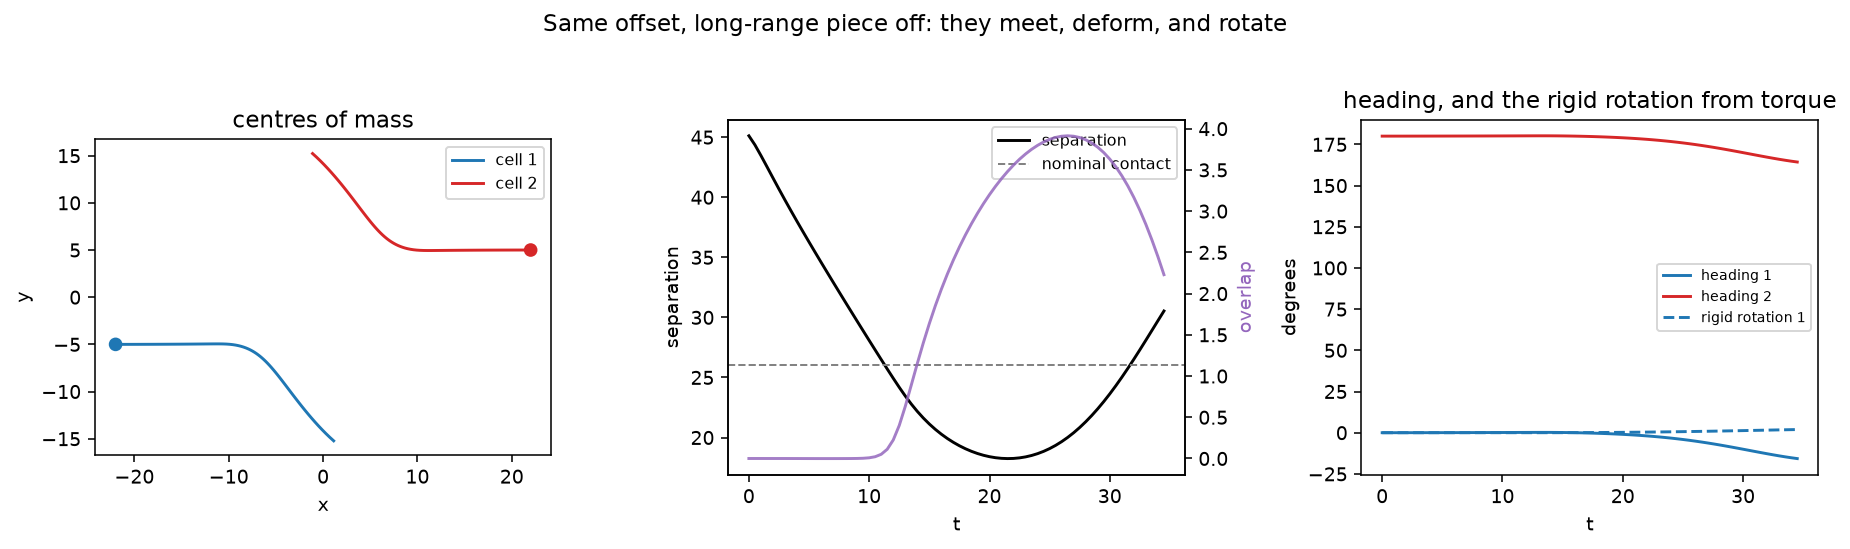
\includegraphics[width=\textwidth]{figures/offset_collision.png}
\caption{Offset approach with the long-range repulsion switched off. Left: centres of mass; the cells meet and then separate. Centre: separation falls through the nominal contact distance (dashed), and the overlap (purple) peaks near 3.9. Right: the headings rotate by about $16^{\circ}$. The dashed curve is the rigid rotation from equation (\ref{eq:torque}), about $1.9^{\circ}$.}
\label{fig:collision}
\end{figure}

\subsection{Avoidance, when the repulsion has a range}
\label{sec:avoid}

With $\lambda=8$ and $k_{\rm soft}=15$, and with the same offset, the cells never meet. The closest approach is 36.8, against a contact distance of 26, and the overlap remains zero. The paths bend apart and each heading turns by $35^{\circ}$ (Figure \ref{fig:avoid}). The rigid rotation accumulated from equation (\ref{eq:torque}) over the same run is $0.28^{\circ}$. The torque is real, and for a cell of this size on a frictional substrate it does not spin the cell by any angle one would see. Repeating the run with anchoring switched off ($\beta=0$) cuts the heading change to $0.4^{\circ}$, while the closest approach stays 36.4 and the overlap stays zero. The cells still miss, because the force on the centres is still there. The turn of the heading is anchoring: the repulsion deforms the edge, and $\mathbf{P}$ is kept normal to that edge, so the treadmilling direction swings away from the partner.

\begin{figure}[ht!]
\centering
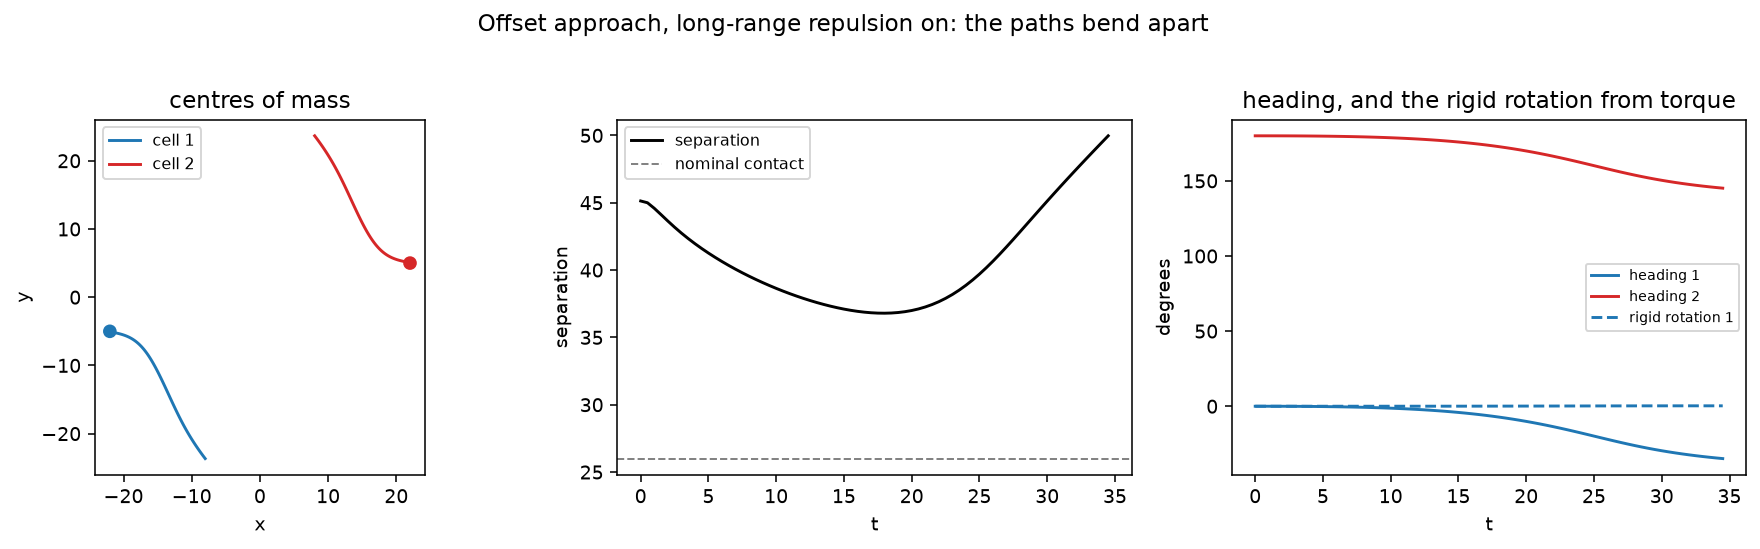
\includegraphics[width=\textwidth]{figures/offset_avoidance.png}
\caption{The same offset approach with the long-range repulsion on. The separation stays above the contact distance (dashed) and the overlap is zero throughout, so it is omitted from the middle panel. The headings turn by $35^{\circ}$. The dashed curve, the rigid rotation from the steric torque, moves by $0.28^{\circ}$.}
\label{fig:avoid}
\end{figure}

Head-on, the offset is removed and symmetry puts the force and both headings on the line of centres. The peak torque over the run is $10^{-6}$, and the accumulated rigid rotation is zero. The centres approach to 28.7, just short of contact, and then recede, with the overlap remaining zero (Figure \ref{fig:headon}). The mean polarization $|\langle\mathbf{P}\rangle|$ falls from 1 to 0.06, while the local magnitude $\langle|\mathbf{P}|\rangle$ dips to about 0.67 and recovers to 0.85. The heading does not rotate. It loses coherence under a sustained head-on load, and by the end of the run it has not reformed into an ordered crawl in a new direction. Reporting the angle of that residual as a reversal would misread a vector whose length is 0.06.

\begin{figure}[ht!]
\centering
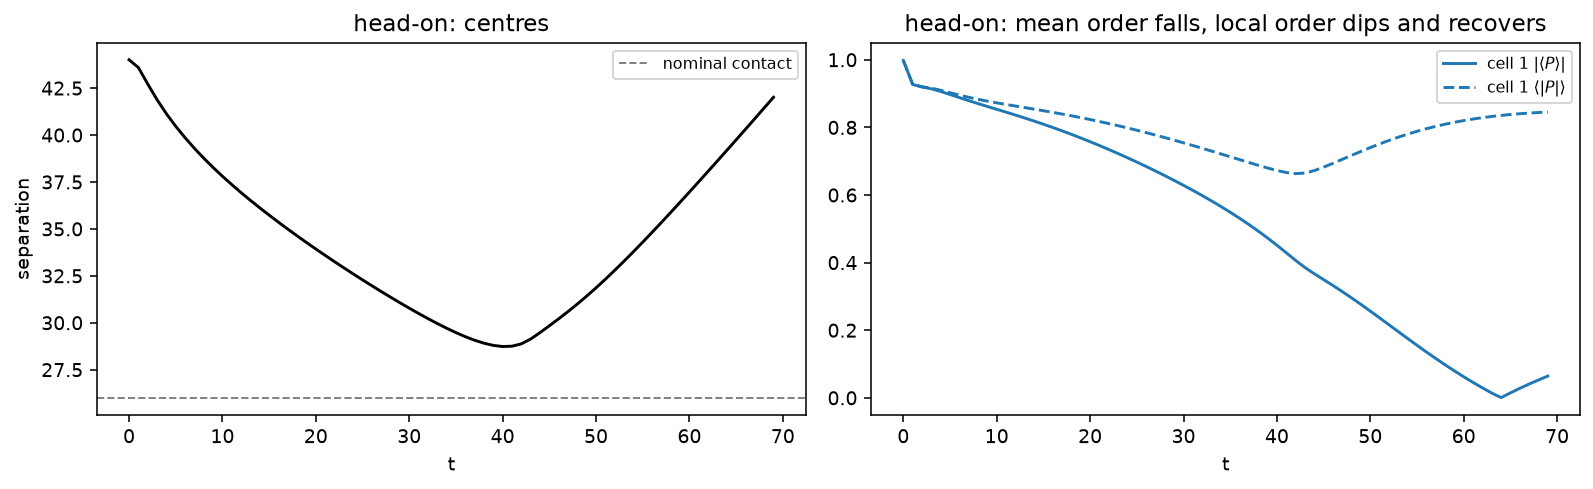
\includegraphics[width=0.92\textwidth]{figures/headon.png}
\caption{Head-on approach with the same long-range repulsion. Left: the centres come in to 28.7 and recede, staying above contact. Right: $|\langle\mathbf{P}\rangle|$ (solid) falls through the compression, while the local order $\langle|\mathbf{P}|\rangle$ (dashed) dips and recovers. The torque on this run is $10^{-6}$.}
\label{fig:headon}
\end{figure}

The cell dependence was checked in two ways. Held fixed and round, with one charge doubled and the shapes unchanged, the force on each cell doubles, from $(11.7,\,2.0)$ to $(23.4,\,3.9)$, and the sum of the two forces is $10^{-11}$. Grown at different radii, $R=13$ and $R=9$, the charges come out at $q=1.02$ and $q=0.50$ because they track the area. On the same offset approach the smaller cell's heading turns by $45^{\circ}$ and the larger cell's by $12^{\circ}$ (Figure \ref{fig:unequal}). The closest separation is 29.5, against a contact distance of 22 for this pair, and the overlap is zero. The force is still equal and opposite. The smaller cell moves more because it has less friction.

\begin{figure}[ht!]
\centering
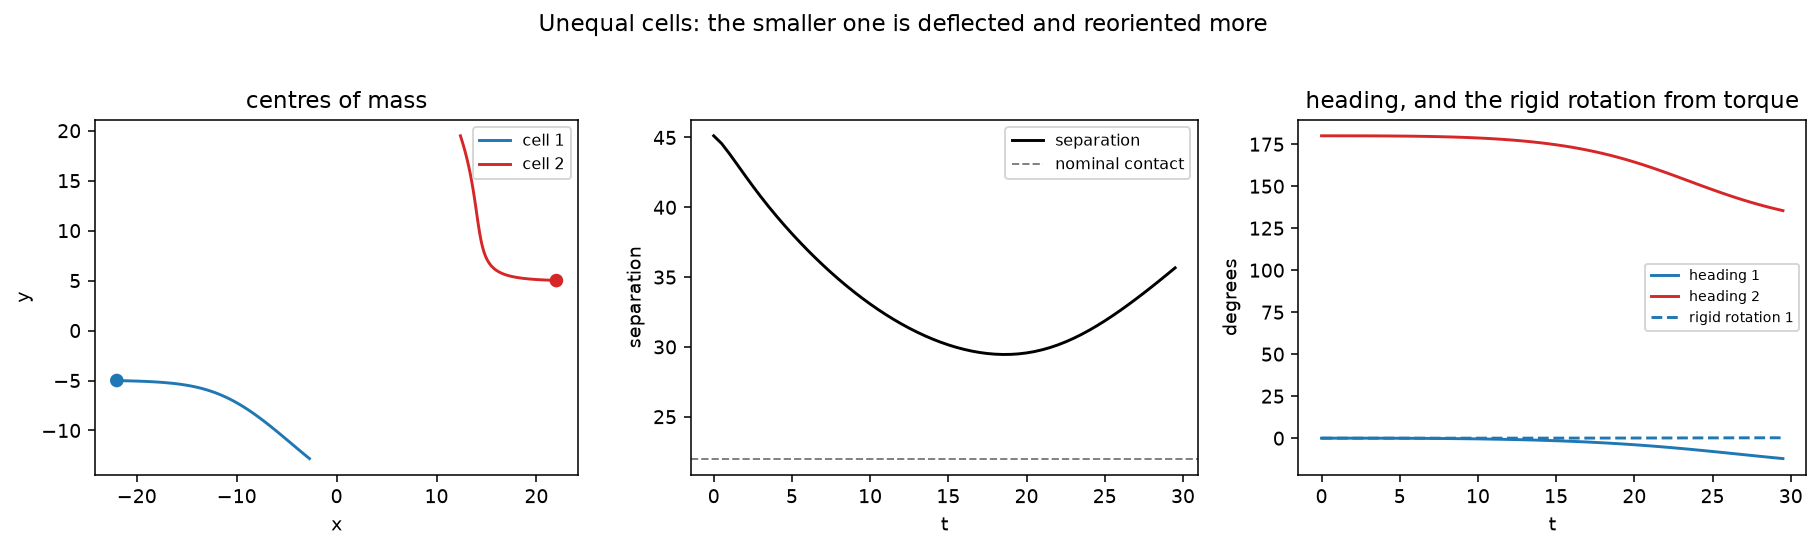
\includegraphics[width=\textwidth]{figures/unequal_cells.png}
\caption{Offset approach between a cell of radius 13 and a cell of radius 9. The smaller cell (red) is thrown further aside and its heading turns by $45^{\circ}$, against $12^{\circ}$ for the larger cell. The overlap stays at zero. The dashed curve is again the rigid rotation, a fraction of a degree.}
\label{fig:unequal}
\end{figure}

Finally the decide--move--relax walk was repeated with equation (\ref{eq:soft}) left on, in the closed box, for a duration of 50. The two cells start aimed at each other. They pass with a closest separation of 28.9 and an overlap of zero, so the collision trigger never fires, and both are still in the move phase at the end. The redirection rule written for a genuine overlap is unchanged from the earlier walk. It simply has nothing to act on in this approach.

\begin{table}[ht!]
\begin{center}
\begin{tabular}{|l|c|c|c|c|}
\hline
Run & Closest sep. & Overlap & Heading & $\int\omega\,dt$ \\
\hline
Offset, $k_{\rm soft}=15$ & 36.8 & 0 & $35^{\circ}$ & $0.28^{\circ}$ \\
Same, anchoring off & 36.4 & 0 & $0.4^{\circ}$ & $0.07^{\circ}$ \\
Offset, $k_{\rm soft}=0$ & 18.3 & 3.9 & $16^{\circ}$ & $1.9^{\circ}$ \\
Head-on, $k_{\rm soft}=15$ & 28.7 & 0 & 0 & 0 \\
Radii 13 and 9 & 29.5 & 0 & $12^{\circ}$, $45^{\circ}$ & $0.23^{\circ}$, $0.13^{\circ}$ \\
\hline
\end{tabular}
\end{center}
\caption{The two-cell runs at the Version 3 parameters. The contact distance is 26 for two cells of radius 13, and 22 for radii 13 and 9. The last column is the rigid rotation from equation (\ref{eq:torque}). Head-on, the torque is $10^{-6}$ and there is no ordered turn. The area of each cell is unchanged to the reported precision in every run.}
\label{tab:twocell}
\end{table}

%%%%%%%%%%%%%%%%%%%%%%%%%%%%%%%%%%%%%%%%%%%%%%%%%%%%%%%%%%%%
%%%%%%%%%%%%%%%%%%%%%%%%%%%%%%%%%%%%%%%%%%%%%%%%%%%%%%%%%%%%
\section{Conclusions}
\label{sec:Conclusion}
%%%%%%%%%%%%%%%%%%%%%%%%%%%%%%%%%%%%%%%%%%%%%%%%%%%%%%%%%%%%
\noindent
The four single-cell stages do what they were built to do. Volume is conserved where the constraint demands it. A treadmilling layer at a wall produces a protrusion and a change of shape with $w_{0}$. The planar model produces the aster and the lamellipodial fan, and the fan is set by anchoring. The friction-dominated reduction crawls at speed 0.801 and is the practical single-cell model, but a collision has to be computed with the shared Stokes solve, because that is the channel through which one cell pushes the other.

Two cells with independent fields and the contact penalty of equation (\ref{eq:contact}) do not merge. In the closed-box walk the overlap reaches 2.07, against about 8.7 for a non-interacting pair at nominal contact, and an off-centre contact with fixed headings rotates each of them by $8.8^{\circ}$. Giving the repulsion a range changes the outcome with the geometry. An offset approach misses, and the heading turns because anchoring follows the deformed edge. A head-on approach cannot turn: the torque vanishes, the cells stop short of contact and separate, and the mean polarization loses coherence instead of rotating. The overdamped balance (\ref{eq:torque}) is the angular statement of the same approximation already made for the linear force. At these parameters it contributes a fraction of a degree on a miss and about two degrees in a hard contact. It is kept, and it is not rescaled to imitate a rigid-body collision.

%%%%%%%%%%%%%%%%%%%%%%%%%%%%%%%%%%%%%%%%%%%%%%%%%%%%%%%%%%%%
%%%%%%%%%%%%%%%%%%%%%%%%%%%%%%%%%%%%%%%%%%%%%%%%%%%%%%%%%%%%
\section{Future scope}
\label{sec:scope}
%%%%%%%%%%%%%%%%%%%%%%%%%%%%%%%%%%%%%%%%%%%%%%%%%%%%%%%%%%%%
\noindent
Three extensions are the natural continuation, and none of them is reported above as a result. The friction $\xi$ is constant, so the biphasic speed of Ref.~\cite{Leoni:2017} cannot appear; a friction that depends on the local speed, together with a cycle in the activity, is the test of that prediction. The pairwise form of equations (\ref{eq:contact}) and (\ref{eq:soft}) extends immediately to more than two cells, by summing every cell's force before the one Stokes solve and adding a steric term for every pair. A four-cell version with an additional tangential contact friction, converting glancing slip into a torque, has been written and has not been run; until those runs exist, no collision angle or overlap is claimed for it. Coupling the vertical slice of Version 2 to the planar solver of Version 3 is what would put the pseudopod and the top-view shapes in a single calculation. The random choice of a new heading after a collision remains a policy. Replacing it by a rule derived from the free energy, rather than imposed, is open, and it should be done only once the measured reorientation at contact is not enough.

\section*{Acknowledgements}
%%%%%%%%%%%%%%%%%%%%%%%%%%%%%%%%%%%%%%%%%%%%%%%%%%%%%%%%%%%%
We thank Prof.\ Sujin B. Babu for suggesting the problem, for the guidance on volume conservation and on the Stokes reduction, and for insisting that a collision be computed with the viscous coupling kept, since two cells push on each other through the fluid.
%%%%%%%%%%%%%%%%%%%%%%%%%%%%%%%%%%%%%%%%%%%%%%%%%%%%

%%%%%%%%%%%%%%%%%%%%%%%%%%%%%%%%%%%%%%%%%%%%%%%%%%%%%%%%%%%%
\begin{thebibliography}{99}
%%%%%%%%%%%%%%%%%%%%%%%%%%%%%%%%%%%%%%%%%%%%%%%%%%%%%%%%%%%%
\bibitem{Bray:2000}
  D.~Bray,
  ``Cell Movements: From Molecules to Motility,''
  2nd ed., Garland Science (2000).
%%%%%%%%%
\bibitem{Verkhovsky:1999}
  A.~B.~Verkhovsky, T.~M.~Svitkina and G.~G.~Borisy,
  ``Self-polarization and directional motility of cytoplasm,''
  Curr.\ Biol.\ {\bf 9}, 11 (1999).
%%%%%%%%%
\bibitem{Keren:2008}
  K.~Keren, Z.~Pincus, G.~M.~Allen, E.~L.~Barnhart, G.~Marriott, A.~Mogilner and J.~A.~Theriot,
  ``Mechanism of shape determination in motile cells,''
  Nature {\bf 453}, 475 (2008).
%%%%%%%%%
\bibitem{Tjhung:2015}
  E.~Tjhung, A.~Tiribocchi, D.~Marenduzzo and M.~E.~Cates,
  ``A minimal physical model captures the shapes of crawling cells,''
  Nat.\ Commun.\ {\bf 6}, 5420 (2015).
%%%%%%%%%
\bibitem{Leoni:2017}
  M.~Leoni and P.~Sens,
  ``Model of cell crawling controlled by mechanosensitive adhesion,''
  Phys.\ Rev.\ Lett.\ {\bf 118}, 228101 (2017).
%%%%%%%%%
\bibitem{Rubinstein:1992}
  J.~Rubinstein and P.~Sternberg,
  ``Nonlocal reaction-diffusion equations and nucleation,''
  IMA J.\ Appl.\ Math.\ {\bf 48}, 249 (1992).
%%%%%%%%%
\bibitem{Ziebert:2013}
  F.~Ziebert and I.~S.~Aranson,
  ``Effects of adhesion dynamics and substrate compliance on the shape and motility of crawling cells,''
  PLoS ONE {\bf 8}, e64511 (2013).
%%%%%%%%%
\bibitem{Yam:2007}
  P.~T.~Yam, C.~A.~Wilson, L.~Ji, B.~Hebert, E.~L.~Barnhart, N.~A.~Dye, P.~W.~Wiseman, G.~Danuser and J.~A.~Theriot,
  ``Actin-myosin network reorganization breaks symmetry at the cell rear to spontaneously initiate polarized cell motility,''
  J.\ Cell Biol.\ {\bf 178}, 1207 (2007).
\end{thebibliography}
%%%%%%%%%%%%%%%%%%%%%%%%%%%%%%%%%%%%%%%%%%%%%%%%%%%%%%%%%%%%
\end{document}
